\section{Methodology}

\begin{figure}
\centering
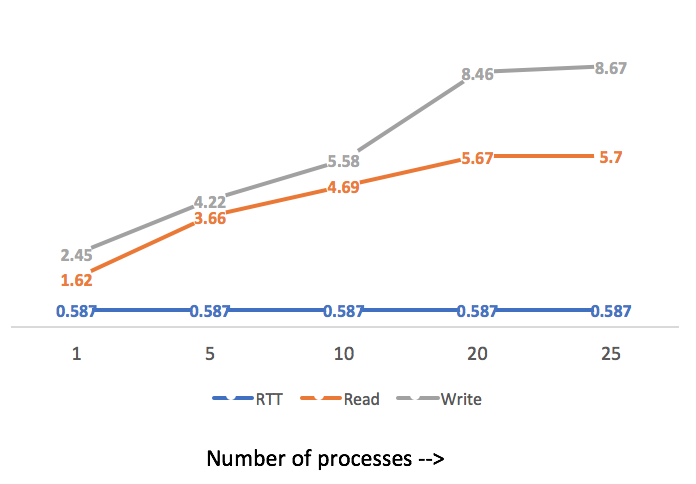
\includegraphics[height=2in, width=3.2in]{images/F_OneClient.png}
\caption{Execution time (in ms) of 1000 READ and WRITE requests generated from each process running in a single client. These requests perform action on the same file.}~\label{fig:figure2}
\end{figure}


Eight servers were rented from the cloud service platform, DigitalOcean, to perform experiments. <Write about server configuration>. We installed Stanford open source implementation of raft, LogCabin, in three of the servers and configured them to run as a Raft cluster. The remaining five servers were used as clients to issue read and write requests to Raft. Fig.\ref{fig:figure1} gives the resultant setup of the model.

The state machine behind the cluster is a file system stored on disk. Each file in the file system stores one single value. These file structures are stored and accessed using tree operations, where the file name is accessed by traversing through the directory structure in the tree. This becomes similar to a key-value store, where the filename and structure is the key which stores a single value. Read requests read the value stored in the file, while write writes or overwrites the value in the file. 

We created read and write files which performs a single read/write or a sequence of reads/writes. Concurrent requests were issued by creating one or multiple processes of these executable read and write files. Hence, if we ran 5 read processes in 5 clients at the same time, each issuing 100 sequential reads, we throw in 25 requests at one time until 100 of such concurrent requests are issued sequentially.



 

